\addcontentsline{toc}{chapter}{Контрольная работа}
\chapter*{Контрольная работа}

\addcontentsline{toc}{section}{Вариант 1}
\section*{Вариант 1}

\subsubsection*{1}

\textit{Задание.} На таможню ежедневно приходит в среднем 10 грузовиков.
Среднее квадратическое отклонение количества грузовиков равно 3.
Используя центральную предельную теорему, найдите такое $x$, что вероятность того,
что за год через таможню пройдёт больше чем $x$ грузовиков, примерно равна $0.99$.

\textit{Решение.}
Обозначим через $ \xi_n$ количество грузовиков, которые прибыли на таможню в $n$-ый день года.
Тогда $S = \xi_1 + \dotsc + \xi_{365}$ является количеством грузовиков,
которые прибыли на таможню за год.
Чтобы найти такое $x$, что $P \left( S > x \right) \approx 0.99$,
воспользуемся аппроксимацией нормальным распределением:
$$P \left( S > x \right) =
  P \left( \frac{S - MS}{ \sqrt{DS}} > \frac{x - MS}{ \sqrt{DS}} \right) \approx
  \Phi_t \left( \frac{x - MS}{ \sqrt{DS}} \right),$$
где $ \Phi_t$ --- функция распределения стандартного нормального распределения.
Значит $x$ находим из условия
$$ \Phi_t \left( \frac{MS - x}{ \sqrt{DS}} \right) \approx
  0.01.$$
Воспользовавшись таблицей значений функции $ \Phi_t$, находим, что
$$ \frac{MS - x}{ \sqrt{DS}} \approx
  2.32.$$
По условию $MS = 365 \cdot M \xi_1 = 3650, \, \sqrt{DS} = \sqrt{365 \cdot D \xi_1} = 3 \sqrt{365}$
и значит $-x + 3650 \approx 2.32 \cdot 3 \sqrt{365} \approx 132.97$,
откуда $x = -132.97 + 3650 \approx 2517$.

\subsubsection*{2}

\textit{Задание.}
Для произвольного действительного числа $y$ вычислите дисперсию $DF_n^* \left( y \right) $,
где $F_n^*$ --- эмпирическая функция распределения, построенная по выборке из распределения $F$.

\textit{Решение.}
$$F_n^* \left( y \right) =
  \frac{1}{n} \sum \limits_{k = 1}^n \mathbbm{1} \left\{ X_k \leq y \right\}, \,
  y \in \mathbb{R}.$$

Ищем дисперсию
$$DF_n^* \left( y \right) =
  D \left( \frac{1}{n} \sum \limits_{k = 1}^n \mathbbm{1} \left\{ X_k \leq y \right\} \right) =
  \frac{1}{n^2} \cdot D \sum \limits_{k = 1}^n \mathbbm{1} \left\{ X_k \leq y \right\}.$$
Вносим дисперсию под знак суммы, пользуясь независимостью случайных величин, а затем используем то,
что они имеют одинаковое распределение
$$ \frac{1}{n^2} \cdot D \sum \limits_{k = 1}^n \mathbbm{1} \left\{ X_k \leq y \right\} =
  \frac{1}{n^2} \sum \limits_{k = 1}^n D \mathbbm{1} \left\{ X_k \leq y \right\} =
  \frac{1}{n^2} \cdot nD \mathbbm{1} \left\{ X_1 \leq y \right\}.$$
Сокращаем константы и пользуемся свойством дисперсии
$$ \frac{1}{n^2} \cdot nD \mathbbm{1} \left\{ X_1 \leq y \right\} =
  \frac{1}{n} \cdot D \mathbbm{1} \left\{ X_1 \leq y \right\} =
  \frac{1}{n} \left[ F \left( y \right) - F^2 \left( y \right) \right] =
  \frac{1}{n} \cdot F \left( y \right) \left[ 1 - F \left( y \right) \right],$$
так как
$M \mathbbm{1} \left\{ X_1 \leq y \right\} =
  1 \cdot P \left( X_1 \leq y \right) + 0 \cdot P \left( X_1 > y \right) =
  P \left( X_1 \leq y \right) =
  F \left( y \right) $,
и $M \left( \mathbbm{1} \left\{ X_1 \leq y \right\} \right)^2 = F \left( y \right) $.

\subsubsection*{3}

\textit{Задание.}
Пусть $X_1, \dotsc, X_n$ --- выборка из нормального распределения $N \left( a, 1 \right) $.
Проверьте несмещённость и состоятельность оценки
$$ \hat{a_n} =
  \frac{ \sum \limits_{i = n + 1}^{2n} X_i}{n}$$
параметра $a$.
Найдите среднеквадратическое отклонение данной оценки от истинного значения параметра $a$.

\textit{Решение.} Проверим несмещённость оценки.
Проверим, выполняется ли $M \hat{a_n} = a$.

Нужно найти математическое ожидание
$$M \frac{ \sum \limits_{i = n + 1}^{2n} X_i}{n} =
  \frac{1}{n} \cdot M \sum \limits_{i = n + 1}^{2n} X_i =
  \frac{1}{n} \sum \limits_{i = n + 1}^{2n} MX_i =
  \frac{1}{n} \left[ 2n - \left( n + 1 \right) + 1 \right] MX_1.$$
Раскрываем скобки
$$ \frac{1}{n} \left[ 2n - \left( n + 1 \right) + 1 \right] MX_1 =
  \frac{1}{n} \left( 2n - n - 1 + 1 \right) MX_1 =
  \frac{1}{n} \cdot na =
  a.$$

Отсюда следует, что оценка несмещённая.

Чтобы дать ответ на второй вопрос задачи,
нужно найти предел по вероятности статистики $ \hat{a_n}$ при $n \to \infty $.
Поскольку случайные величины $X_1, \dotsc, X_n$
являются независимыми одинаково распределёнными случайными величинами с конечным первым моментом,
то согласно закону больших чисел
$$ \frac{1}{n} \sum \limits_{i = n + 1}^{2n} X_i \overset{P}{ \rightarrow } MX_1, \,
  n \to \infty,$$
а тогда при $n \to \infty: \, \hat{a_n} \overset{P}{ \rightarrow } MX_1 = a$.

Значит статистика $ \hat{a_n}$ является состоятельной оценкой параметра $a$.

Формула среднеквадратического отклонения имеет вид $ \sigma = \sqrt{D \xi }$.

Найдём дисперсию оценки
$$D \frac{ \sum \limits_{i = n + 1}^{2n} X_i}{n} =
  \frac{1}{n^2} \cdot D \sum \limits_{i = n + 1}^{2n} X_i =
  \frac{1}{n^2} \cdot nDX_1 =
  \frac{1}{n} \cdot DX_1 =
  \frac{1}{n}.$$

Извлекая корень, получаем
$$ \sigma =
  \sqrt{ \frac{1}{n}} =
  \frac{1}{ \sqrt{n}}.$$

\subsubsection*{3}

\textit{Задание.} Пусть $X_1, \dotsc, X_n$ --- выборка из распределения Бернулли.
Является ли статистика $p_n^* = \left( \overline{X} \right)^2$ несмещённой оценкой параметра $p$?
Состоятельной?

\textit{Решение.}
Для того, чтобы выяснить, является ли статистиа $p_n^*$ несмещённой оценкой параметра $p$,
необходимо проверить, выполняется ли условие $Mp_n^* = p$.
Находим математическое ожидание статистики $p_n^*:$
$$Mp_n^* =
  M \left( \overline{X} \right)^2 =
  M \left( \frac{1}{n} \sum \limits_{i = 1}^n X_i \right)^2 =
  \frac{1}{n^2} \cdot M \left( \sum \limits_{i = 1}^n X_i \right)^2.$$
По свойствам дисперсии
$$ \frac{1}{n^2} \cdot M \left( \sum \limits_{i = 1}^n X_i \right)^2 =
  \frac{1}{n^2} \cdot D \sum \limits_{i = 1}^n X_i +
  \frac{1}{n^2} \cdot \left( M \sum \limits_{i = 1}^n X_i \right)^2.$$
Воспользуемся тем, что случайные величины независимы и одинаково распределены
$$ \frac{1}{n^2} \cdot D \sum \limits_{i = 1}^n X_i +
  \frac{1}{n^2} \cdot \left( M \sum \limits_{i = 1}^n X_i \right)^2 =
  \frac{1}{n^2} \cdot nDX_1 + \frac{1}{n^2} \cdot \left( nMX_1 \right)^2.$$
Сокращаем константы
$$ \frac{1}{n^2} \cdot nDX_1 + \frac{1}{n^2} \cdot \left( nMX_1 \right)^2 =
  \frac{1}{n} \cdot DX_1 + \left( MX_1 \right)^2 =
  \frac{1}{n} \cdot \sqrt{p} \left( 1 - \sqrt{p} \right) + p.$$

Таким образом
$$Mp_n^* =
  \frac{1}{n} \cdot \sqrt{p} \left( 1 - \sqrt{p} \right) + p \neq
  p,$$
а значит статистика $p_n^*$ не является несмещённой оценкой неизвесного параметра $p$.

Чтобы дать ответ на второй вопрос задачи,
нужно найти предел по вероятности статистики $p_n^*$ при $n \to \infty $.
Поскольку случайные величины $X_1, \dotsc, X_n$
являются независимыми одинаково распределёнными случайными величинаим с конечным первым моментом,
то согласно закону больших чисел
$$ \frac{1}{n} \sum \limits_{i = 1}^n X_i \overset{P}{ \rightarrow } MX_1, \,
  n \to \infty,$$
а тогда при $n \to \infty: \, p_n^* \overset{P}{ \rightarrow } \left( MX_1 \right)^2 = p$.
Значит статистика $p_n^*$ является состоятельной оценкой параметра $p$.


\subsubsection*{5}

\textit{Задание.}
Найдите оценку максимального правдоподобия параметра
$$ \theta >
  0,$$
если распределение выборки имеет плотность
$$p \left( y \right) =
  \frac{2y}{ \theta } \cdot \mathbbm{1} \left\{ y \in \left[ 0, \theta \right] \right\}.$$

\textit{Решение.} Согласно методу максимального правдоподобия,
в качестве оценки несмещённого параметра $ \theta $ выбирается статистика $ \theta^*$,
которая даёт наибольшее значение функции правдоподобия, которая для данной выборки имеет вид
$$L \left( X_1, \dotsc, X_n, \theta \right) =
  \prod \limits_{i = 1}^n
    \frac{2X_i}{ \theta } \cdot \mathbbm{1} \left\{ X_i \in \left[ 0, \theta \right] \right\} =
  \frac{2^n \prod \limits_{i = 1}^n X_i}{ \theta^{n}} \cdot
  \mathbbm{1}
    \left\{ X_{ \left( 1 \right) } \geq 0, \, X_{ \left( n \right) } \leq \theta \right\}.$$

Заметим, что функция правдоподобия не дифференцируема по $ \theta $.

Из  приведённого на рисунке \ref{fig:5} графика функции $L$ как функции переменной $ \theta $
делаем вывод, что максимального значения она достигает в точке $X_{ \left( n \right) }$.
Значит оценкой максимального правдоподобия является статистика $ \theta^* = X_{ \left( n \right) }$.

\begin{figure}[h!]
  \centering
  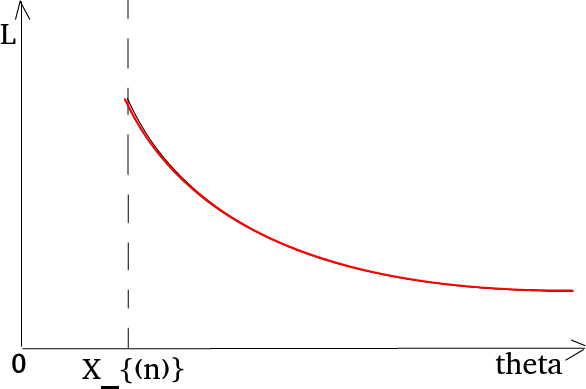
\includegraphics[width=.4\textwidth]{./pictures/v1_5.png}
  \caption{Функция правдоподобия}
  \label{fig:5}
\end{figure}
